

%%%%%%%%%%%%%%%%%%%%%%%%%%%%%%%%%%%%%%%%%%%%%%%%%%%%%%%%%%%%%%%%%%%%
%% I, the copyright holder of this work, release this work into the
%% public domain. This applies worldwide. In some countries, this may
%% not be legally possible; if so: I grant anyone the right to use
%% this work for any purpose, without any conditions, unless such
%% conditions are required by law.
%%%%%%%%%%%%%%%%%%%%%%%%%%%%%%%%%%%%%%%%%%%%%%%%%%%%%%%%%%%%%%%%%%%%

\documentclass[
  digital, %% This option enables the default options for the
           %% digital version of a document. Replace with `printed`
           %% to enable the default options for the printed version
           %% of a document.
  table,   %% Causes the coloring of tables. Replace with `notable`
           %% to restore plain tables.
  lof,     %% Prints the List of Figures. Replace with `nolof` to
           %% hide the List of Figures.
  lot,     %% Prints the List of Tables. Replace with `nolot` to
           %% hide the List of Tables.
  %% More options are listed in the user guide at
  %% <http://mirrors.ctan.org/macros/latex/contrib/fithesis/guide/mu/fi.pdf>.
  oneside
]{fithesis3}
%% The following section sets up the locales used in the thesis.
\usepackage{listings}
\usepackage[resetfonts]{cmap} %% We need to load the T2A font encoding
\usepackage[T1,T2A]{fontenc}  %% to use the Cyrillic fonts with Russian texts.
\usepackage[
  main=english, %% By using `czech` or `slovak` as the main locale
                %% instead of `english`, you can typeset the thesis
                %% in either Czech or Slovak, respectively.
 %english, german, russian, czech, slovak %% The additional keys allow
]{babel}        %% foreign texts to be typeset as follows:
%%
%%   \begin{otherlanguage}{german}  ... \end{otherlanguage}
%%   \begin{otherlanguage}{russian} ... \end{otherlanguage}
%%   \begin{otherlanguage}{czech}   ... \end{otherlanguage}
%%   \begin{otherlanguage}{slovak}  ... \end{otherlanguage}
%%
%% For non-Latin scripts, it may be necessary to load additional
%% fonts:
\usepackage{paratype}
\bibliographystyle{unsrt}
\usepackage{hyperref}
\usepackage[
   backend=biber        % if we want unicode
  ,style=numeric % or iso-numeric for numeric citation method
  ,autolang=other       % to support multiple languages in bibliography
  ,sortlocale=cs_CZ     % locale of main language, for sorting
  ,bibencoding=UTF8     % this is necessary only if bibliography file is in different encoding than main document
]{biblatex}

\def\textrussian#1{{\usefont{T2A}{PTSerif-TLF}{m}{rm}#1}}
%%
%% The following section sets up the metadata of the thesis.
\thesissetup{
    date          = \the\year/\the\month/\the\day,
    university    = mu,
    faculty       = fi,
    type          = mgr,
    author        = Tomáš Šíma,
    gender        = m,
    advisor       = {RNDr. Martin Stehlík},
    title         = {Darknet market analysis and user de-anonymization},
    TeXtitle      = {Darknet market analysis and user de-anonymization},
    keywords      = {blockhain, bitcoin, darknet, drug market, TOR, cryptocurrency, anonymity, metadata, de-anonymizatio
n},
    TeXkeywords   = {blockhain, bitcoin, darknet, drug market, TOR, cryptocurrency, anonymity, metadata, de-anonymizatio
n},
    abstract      = {This thesis has two goals. First goal is to perform quantitative statistical analysis of
    Valhalla cryptomarket. We scraped Valhalla cryptomarket website for information about vendors, listings and buyers
    and brought up a lot of interesting statistics about them.
    
    The second goal of this thesis is to create a tool to find, analyze and visualize publicly available data,
 which can be helpful to deanonymize users of drug markets available via TOR on dark web. The aim of this tool is to help investigators with collecting intelligence on entities related to these drug markets. Users and operators of these markets employ multiple means to prevent their deanonymization. Cryptomarkets are operated ad TOR services, PGP encryption is often required to communicate between multiple parties and bitcoin is used as a way to pay for goods or services.
 
    We scraped multiple publicly available social sites and websites related to bitcoin(Twitter, Bitcointalk, Reddit,
    blockchain.info...) and drug markets themselves using python.
    We stored all these data into neo4j database, which is a graph database based on PostgreSQL.
    We created a tool, which uses these data and multiple heuristics to analyze and visualize data and metadata of users
, drug markets, social media and blockchain.
    The tool can also for given address find the nearest addresses or transactions related to drug markets and also find the nearest addresses that are mentioned in scraped websites. 
    
    To test the efficiency of this tool, we created multiple profiles on these dark markets and performed multiple transactions to deposit and withdraw bitcoins. 
    },
    thanks        = {I would like to thank my supervisor RNDr. Martin Stehlík Ph.D. for guiding me and providing technical support for my work. 
    
    I would also like to thank Mgr. Jaroslav Šeděnka for his continuous stream of helpful comments and ideas.
    
    Access to computing and storage facilities owned by parties and projects contributing to the National Grid Infrastructure MetaCentrum provided under the programme "Projects of Large Research, Development, and Innovations Infrastructures
" (CESNET LM2015042), is greatly appreciated.},
    bib           = citations.bib
}

\usepackage{makeidx}      %% The `makeidx` package contains
\makeindex                %% helper commands for index typesetting.
%% These additional packages are used within the document:
\usepackage{paralist} %% Compact list environments
\usepackage{amsmath}  %% Mathematics
\usepackage{amsthm}
\usepackage{amsfonts}
\usepackage{url}      %% Hyperlinks
\usepackage{markdown} %% Lightweight markup
\usepackage{listings} %% Source code highlighting
\usepackage{graphicx}
\graphicspath{ {images/} }
\lstset{
  basicstyle      = \ttfamily,%
  identifierstyle = \color{black},%
  keywordstyle    = \color{blue},%
  keywordstyle    = {[2]\color{cyan}},%
  keywordstyle    = {[3]\color{olive}},%
  stringstyle     = \color{teal},%
  commentstyle    = \itshape\color{magenta}}
\usepackage{floatrow} %% Putting captions above tables
\usepackage{geometry}
\usepackage{pythontex}

\floatsetup[table]{capposition=top}
\begin{document}
\setpygmentsfv{xleftmargin=4ex}
\chapter{Introduction}
%\addcontentsline{toc}{chapter}{Introduction}

The relative anonymity of internet offers an incentive for criminal parties to use the internet as a tool for their activities.
Internet facilitated some forms of existing crimes (selling drugs, guns and
counterfeits, running Ponzi schemes) and also enabled many new types of frauds like hacking, phishing, carding and identity theft.

Publicly available statistics show, that cybercriminals are much
 less likely to be discovered and persecuted.
 In USA in 2010, there were 5628 robberies and the loot was recovered in more than 20\% cases. \parencite{fbi10} 
 FBI recieved 303809 complaints related to cyber crime in 2010, resulting in just 6 convictions. \parencite{fbcyber} 
Criminals value their anonymity very high and use various means to prevent them from being caught by police forces.
\parencite{tzanetakis2016transparency}
\parencite{van2013surfing}
\parencite{aldridge2014not}

A big problem for criminals was getting the money they got from criminal activity to their possession,
since that required some form of physical presence or identification.
Also, it was hard for two anonymous entities engaging in criminal activity to transfer value to each other,
 because it's hard to setup anonymous bank account and neither party could be sure about the origin of
 the money they are receiving.

For bitcoin, there is no central authority requiring bitcoin address
(bitcoin equivalent of bank account number) to be linked to person's identity and so 
criminals can use their anonymous connection to the internet to both receive and send bitcoins without disclosing their identity.
However, all bitcoin transactions are publicly available and so each bitcoin can be tracked through the whole transaction history.
 Cryptomarkets are online marketplaces with listings offering illegal goods and services.
 Cryptomarkets are accessible via TOR network and users of cryptomarkets use PGP to communicate. 
n history. These mechanisms make it possible for cryptomarkets to publicly operate, yet be hard to reach by law enforcement.
\parencite{cox2016staying}

We scraped and examined data from Valhalla market,
 one of the most popular and well established currently (February 2018) operating drug markets,
in order to do a statistical analysis of the scale of its operations.

We collected data from multiple public sources related to drug markets and bitcoin transactions and explored
 possibilities to de-anonymize drug market's users by linking publicly known identities to nearby bitcoin addresses.
We also created a tool to visualize data obtained from these public sources and search for nearby bitcoin addresses.

\section{Goals}

The main goal of this thesis is to analyze Valhalla drug market
and try multiple approaches to deanonymize users related to this drug market.
The results of this work are data from cryptomarket and
 showing interesting statistics about the whole market as well as actors operating there.
 Also, we gathered addresses tied to some form of identification, like usernames, from social networks and publicly available forums.
Another goal of this work is to create a tool, that uses the data mentioned above to help the investigator to disclose transactions
, Bitcoin addresses and identities related to online drug markets.

We managed to partly fill our goals. We successfully scraped data from cryptomarket and did an analysis.
We scraped data about identities linked to bitcoin addresses and created a tool to visualize them.
We were just partly successful with finding heuristics, that would cluster multiple bitcoin addresses belonging to the
same owner.

\section{Structure of thesis}
XXX - mozna se zmeni lehce jmena/poradi kapitol, jinak povidani stejne

The following text describes individual chapters of this thesis.
Chapter Related works give an overview of works already done on similar topics. 

Chapter Technology and terms starts with a quick introduction to bitcoin and blockchain,
which is used for paying on crypto markets.
It also describes how cryptomarkets work and tools that are used by cryptomarkets' users and administrators.

The chapter Methods and tools describes the process of collecting and storing the data from bitcoin blockchain,
drug markets and publicly available forums and social networks. 

Deanonymization techniques chapter describe heuristics and methods that are later used by the application to detect 
addresses used by drug markets and link the users of drug markets to publicly found identities.

Chapter Statistics of drug markets consists of various statistics about drug markets, that were gathered during drug mar
ket website scraping.
It contains two parts, the first is focused on statistics related to cash flows, the second part is giving insight about
 non-money related statistics.

The chapter called Application describes the functionality, implementation, usage and 
possible future development of the application for investigating bitcoin addresses, which was created as part of this thesis
.

Testing and verification is about the testing of the created application.
The last chapter is a discussion about achieved goals, problems of implementation and possible future improvements.

\chapter{Related terminology}

In this chapter, I explain the terms and technology related to online drug markets.
The online drug markets use several technologies, that are crucial to their anonymous operation.
The Bitcoin enables different parties to exchange value in an anonymous way.
TOR allows users and administrators of a marketplace to hide from any third party doing packet sniffing on the network,
that they are accessing drug marketplace. It also hides the location on drug marketplace web server from its users.
PGP enables sellers and vendors to communicate between each other in an encrypted way,
so that drug market administrators cannot eavesdrop on that communication.
Drug markets also use bitcoin mixers, services designed to mix their funds with others, in order to obstruct
analysis of their cash flow and improve anonymity of users and administrators.

\section{Bitcoin and blockchain}

Bitcoin \parencite{nakamoto2008bitcoin} is the first decentralized peer to peer cryptocurrency,
created by the anonymous author(s) known by pseudonym Satoshi Nakamoto in 2008.
Bitcoin transactions are not verified by the central authority, they are processed by distributed peer to peer network of bitcoin nodes instead. 
The source code of bitcoin nodes is open source and can be downloaded and run locally. 
The entire history of transactions is stored in a distributed public ledger called blockchain.
Bitcoin combines multiple cryptography algorithms to achieve consensus among nodes
on the state of the blockchain. Anything once written in the blockchain
cannot be removed or modified. State of blockchain can be modified only in that way, that new
block of transactions is added at the end of the blockchain.

\subsection{Addresses, bitcoins and transactions}
In order to receive and send bitcoins, a user needs to have a bitcoin address.
A bitcoin address is simply a BASE58 encoded public key with 4 bytes added for checksum.
Each address has it's associated private key.
In order to send bitcoin from bitcoin address, a user needs to have a private key associated with the given bitcoin address.
Storing and using bitcoin addresses and associated private keys is automatically managed
by software called bitcoin wallet. There exist many third party software wallets.

All the transactions, bitcoins and addresses are stored in the blockchain,
the balance of all addresses and all transactions are publicly available.
In order to not see the whole history of transactions of address's owner,
the bitcoin wallets generate new bitcoin address for each new incoming transactions. When spending bitcoins, it use one or more of the addresses the wallet generated previously.
Therefore, when pairing the address to identity, we can directly obtain just the history of transactions related to the given
address, but can not get all transactions and balance of the user, as he is likely to own multiple bitcoin addresses.

Bitcoins in blockchain are represented as inputs and outputs of the transaction.
Each transaction has some inputs and outputs. 
Input and output is the same data structure, it only differs in it's relationship to given transaction.
Each input/output consists of its unique identifier, its value in bitcoins and bitcoin address that owns it.
Every output can be used exactly once as an input of new transaction, and therefore the owner of output can not
spend one output multiple times.

When the sender sends bitcoin to recipient, he generates a transaction.
The new transaction must satisfy:
\begin{itemize}
  \item He owns address of the inputs = He can spend only bitcoins he owns
  \item Each input has not been used as input in any other transaction = He cannot spend one output multiple times
  \item The sum of bitcoins of transaction's inputs is equal to the sum of bitcoins of transaction's output + fees
\end{itemize}

The new transaction must have 1 or more outputs.
There can be multiple outputs in a transaction with different associated addresses and bitcoin value,
however, there happens to be a common pattern. When the sender sends bitcoins to one recipient,
the transaction contains two outputs.
One output contains recipient's address and the volume of bitcoins he receives.
One output is called "change output". Because sender usually doesn't own outputs that sum to be equal to the number of bitcoins he wants to send, he adds a second output to the transaction. The second output has an address he owns and amount of bitcoins, he will receive from the transaction back.
 This is the only way to split bitcoins into smaller parts. 

When sending transaction,
 wallet software creates transaction data and signs it with keys of addresses that are sending the bitcoins.
 Then it sends it to one or multiple bitcoin nodes.
Nodes collect transactions from users and broadcast them to other nodes on best effort basis.
The validity of the transaction is later checked by miners and if everything is ok, they add it to the blockchain.

\subsection{Mining}

Miners are verifying transactions.
Miners are running bitcoin nodes and mining software, which enables them to create a new block of transactions, add it to blockchain and broadcast new, longer version, of blockchain to other nodes.
Finding a new block of transactions is a hard problem from computational perspective.
Miners look for a solution to the problem by brute-force and when they find a solution, they are able to generate a new block of transactions. The difficulty of the problem is adjusted every 2016 block,
so that new block is generated on average every 10 minutes.

Some of the variables for the problem are dependent on the last block in the blockchain, so it is impossible
to precompute the problem for blocks that will come in the future. 
Miner and anyone else knows the definition of the problem just for the block that will immediately follow.

When miner generates a new block, he can claim all of the fees of transactions included in that block,
also he is able to create a special transaction called coinbase transaction, that sends bitcoins from nowhere to his address. By these coinbase transactions, new bitcoins are emitted into the network.
He also broadcast his new block, so other miners can update their blockchains. 

\section{TOR - the onion routing}

Tor \parencite{dingledine2004tor} is a free open source software, that provides access to Tor network. Tor network is a network of Tor nodes.
The goal of Tor project is to provide it's users encrypted access to the internet in order to prevent third parties
from eavesdropping and analysis of the transmitted data.
The communication of the user's computer with the network is encrypted and rerouted through multiple Tor nodes using onion routing technology.
The usage of Tor can be detected by the third party, but the third party can not decrypt user's data, that are transmitted
 via TOR.
Some websites restrict access from TOR, due to many risks involved.

Communication between browser and web server is usually done via HTTPS protocol.
This protocol uses asymmetric cryptography. The web server and browser exchange their public keys at the start of communication
and encrypt the data using these keys. Decrypting the data is possible only by corresponding private keys,
which the browser and web server keep locally. This protocol is susceptible to man in the middle attacks.
If the attacker has control over the transmission from the start of communication, he can place himself in the middle of communication and act as a web server for user and as a user for the web server. To prevent these types of attack,
 a certification authority is needed. The certification authority is an institution, that sign public keys, belonging to the web server.
 When the browser receives the public key, it automatically checks, if it is signed by any authority from its list of authorities and if not, it displays warning or error message.
 
The HTTPS protocol encrypts data, but doesn't hide the identity of the user from the web server,
 and also the internet provider can see, where is the user connecting to.
 In TOR, the user's identity is hidden from the web server, and internet provider can only see, that user is connecting to TO
R, but can not see where is the destination of the data that are transmitted via TOR.
 Tor uses Onion routing technology. When a user visits a website, there TOR software picks randomly few TOR nodes from the network and establish a circuit, as we can see on \ref{TOR routing schema}. 
 The packet of data is encrypted with each public key of the node in the circuit, starting from the last node as on \ref{TOR
 packed encryption schema}.
 No TOR node knows the whole path of the packet, only his neighbour nodes on the path.
 The TOR node knows the previous node he received the packet from. It gets also the address 
 of next node by decrypting the packet and reading the added metadata.
 
 \begin{figure}[!htb]
    \centering
    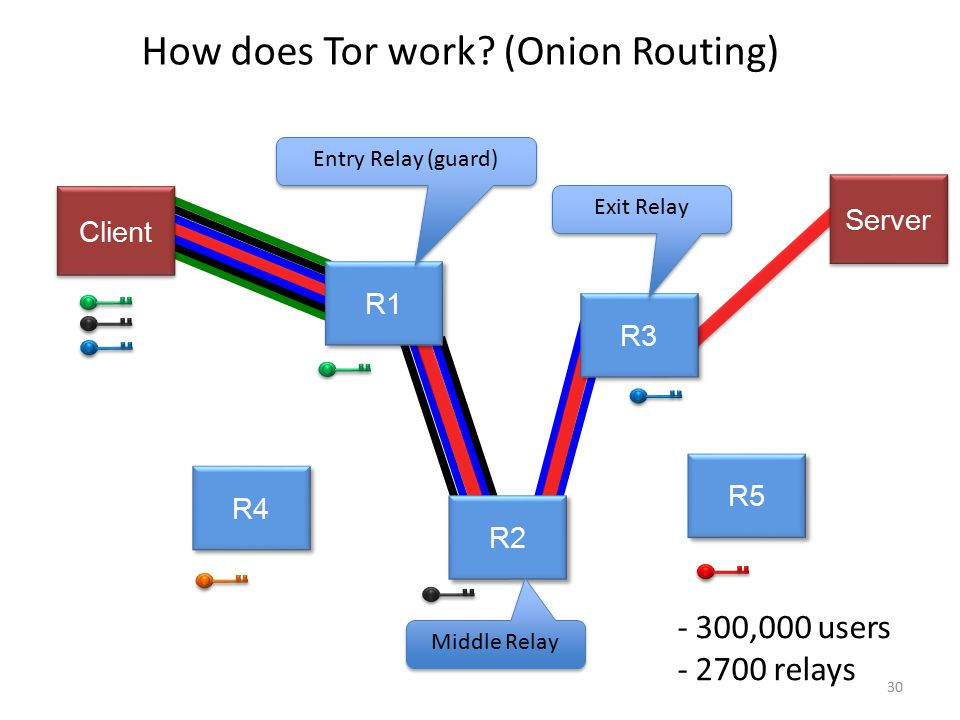
\includegraphics[width=1\textwidth]{tor-prejate}
    \caption{TOR routing schema}
    \label{TOR routing schema}
\end{figure}
 
  \begin{figure}[!htb]
    \centering
    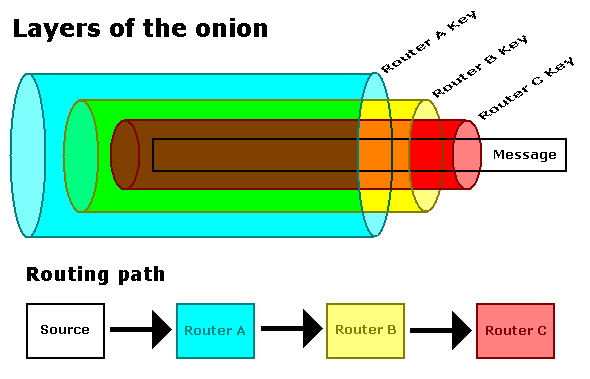
\includegraphics[width=1\textwidth]{tor-packet-prejate}
    \caption{TOR packed encryption schem}
    \label{TOR packed encryption schema}
\end{figure}
 
\section{PGP}

PGP \parencite{Zimmermann:1995:OPU:202735} is a program for encrypting data
and communication between two parties using public key cryptography.
PGP is used for signing, encrypting and decrypting messages, mostly e-mails.
PGP was developed in 1991 as open source, with the intention 
to provide an open widely used standard for encrypted communication.
Nowadays, PGP program is not open source anymore, but the standard is used by open source GPG software.

PGP uses public key cryptography. Unlike symmetric cryptography, public key cryptography
uses two different keys for encrypting and decrypting.
A user generates a pair of keys, a public key for encrypting emails sent to him and private key, which the user
 keeps for himself and uses for decrypting messages encrypted with the associated public key.
 The user also publishes his public key, so other users can send him encrypted messages.

PGP is used in the context of online drug markets as a means of communication between vendors and customers.
Both vendor and customer have their public keys published on their profile page and use the public key of the other
party to encrypt messages to them. This enables vendors and sellers to keep their communication private also from the administrators of the marketplace.

\section{Cryptomarkets}

Illegal online markets have been around for more than 30 years \parencite{motoyama2011analysis}.
On these markets, users can sell and buy drugs, weapons, hacking tools, stolen credit cards,
counterfeit currency, forged documents and other illegal goods and services.
Most markets forbid selling the most unambiguously harmful goods, such as child pornography or hitman services.
 
In 2011 appeared a new type of illegal online marketplace called cryptomarket. 
A cryptomarket is an illegal online market accessible only via TOR network and using bitcoins
as a means of making payments. These two technologies provided a safer environment
than previous markets hosted on forums and chatrooms.

Physical products, like drugs, are sent to buyer via ordinary mail to address provided by the buyer.
The package is disguised as packages containing common goods sent by big online retailers.
\parencite{paquet2017cryptomarkets}

Cryptomarkets are popular with vendors,
because they offer high traffic, secure and anonymous environment for conducting their bussiness\parencite {van2014responsible}.
Cryptomarkets offer safer, more comfortable and more professional way of buying drugs, avoiding 
the need to meet face to face with dealers \parencite{barratt2014use}.

Nowadays, there exist multiple cryptomarkets competing against each other and the risk
of a failure of a deal is still high \parencite{wehinger2011dark}.
In order to protect buyers, cryptomarkets use Escrow and vendors' feedback to identify scammers and minimize losses.
Cryptomarkets also use Tumbler services, which makes it harder to detect and analyze bitcoin transactions
 related to these illegal activities.

\subsection{The process of ordering}
Most of the supermarkets are publicly available and there is no fee
for creating a user account. The act of buying drugs from them is considered user-friendly by buyers and is nearly identical to the process of buying goods from popular lawfull e-shops like Amazon.

 The whole process consists roughly of these steps:
\begin{enumerate}
\item User creates an account on cryptomarket if he doesn't have one already
\item He top up his account by sending bitcoins to the bitcoin address,
that was generated for his deposits.
\item He than find an offer, that he is interested in and buy it in a similar
way as in any other e-shop.
\item Buyers money is now locked by cryptomarket.
\item Buyer and vendor communicate out the way of delivery.
\item If the buyer receives goods or services, he confirms it and money is unlocked to the vendor.
\item Buyer gives feedback to the vendor. 
\end{enumerate}

Vendors value their feedback ratings very high, so they encourage buyers to leave
 positive feedback when the transaction goes well.
 
\subsection{Tumbler}
Bitcoin transactions are publicly available, but it is not easy to identify their owners.
It might seem, that bitcoin transactions are anonymous, but when user send bitcoins to
someone(exchange) who knows their identity, the recipient can pair the bitcoin address
the bitcoins came from to identity of the sender.
Although bitcoin users usually use multiple bitcoin addresses,
their transactions and addresses are still 
susceptible to blockchain cashflow analysis,
which might identify other addresses of the owner of address we already know.

Bitcoin Tumblers exist in order to prevent such analysis.
A user sends bitcoins to the tumbler service, the service mix his bitcoins
with bitcoins of other users by performing multiple transactions
between its bitcoin addresses. \parencite{moser2013inquiry}
  
The structure of these transactions differs for different tumbler services.
User send their bitcoins to address owned by the tumbler,
then he generates new bitcoin address with no tie to his previous addresses
and receives bitcoins from tumbler service to his new bitcoin address.
 There also exists peer-to-peer tumblers(CoinJoin, SharedCoin, Coinswap),
that enable multiple users to directly create transactions to mix bitcoins among themselves.
Transactions can be performed multiple types with different actors.

\subsection{Vendor's feedback}

Cryptomarkets usually employ reputation systems,
where buyers can share their satisfaction with vendors.
These systems are similar to systems used in popular e-commerce websites like Amazon or Ebay.
Users can give feedback only to vendors with whom they have traded with.
On some cryptomarkets, it is only possible to upvote and downvote vendors,
on some others, people can rate different parts of their interaction with the seller,
like the easiness of communication,
the speed of sending the goods and unsuspiciousness of packaging.

Feedback is not mandatory, but vendors encourage buyers to give them positive feedback
\parencite{aldridge2014not}\parencite{soska2015measuring}, because the positive feedback
ratio gives vendor significant advantage over vendors with worse feedback.

\subsection{Valhalla cryptomarket}

We selected Valhalla cryptomarket based on three metrics.
The first metric is its size. Valhalla market is well known operating cryptomarket.
It has more than 20 000 active listings and 600 vendors.
This is the second most listings and vendors, just behind dream market.

Among significant cryptomarkets (dream market, Point market, Wall Street Market), Valhalla
has been operating for the longest time. This is to advantage of our analysis, as we can analyze matured cryptomarket with vendors, who have been selling for a longer time and have more reviews.

Among cryptomarkets mentioned above,
Valhalla cryptomarket provides the most information about vendors and buyers.
The feedback page of given vendor consists of feedbacks, where
each given feedback contains comment when the feedback was given,
what was the listing the user gave feedback for, what was the price,
the amount, how much the buyer bought overall on the Valhalla market,
how many trades have buyer done and first, last 2 digits of the buyer.

The 2 first and last digits of buyer's username are really unique for Valhalla market,
other markets offer first and last character of buyer's username at most.
This will drastically help with recognizing the same buyer among multiple reviews.
The fact, that feedback also contains related listing allows us to
detect, which vendor's listings are popular and earning the most money for the vendor.

\chapter{Related works}
\section{Blockchain analysis and linking bitcoin addresses}

Multiple papers and tools were published regarding the analysis of blockchain.
Blockchain contains all bitcoin transactions and anyone can simply check,
the source and destination addresses of every transaction in the system.
It is heavily encouraged for users of blockchain to use multiple bitcoin addresses
 and every major bitcoin wallet (software, for receiving and sending bitcoins) do so.
 It is a big challenge to cluster addresses belonging to the same user.
 
The authors of first research article \parencite{reid2013analysis}
 parsed blockchain files to create a graph of bitcoin transactions, with vertices as transactions
 and edges between them represented bitcoins flowing from one transaction to another.
 They created so-called user graph by clustering addresses belonging to the same user.
 They used simple heuristics, that the owner of all input addresses used in a transaction must be the same. The first version of this article  
was published in 2011 and dealt with a much smaller number of people using bitcoin and smaller transaction graph.
Their analysis also focuses on deanonymization through multiple aspects of bitcoin protocol,
while this thesis focuses on deanonymization from transaction graph and public data.

Androulaky \parencite{androulaki2013evaluating} performed clustering using two heuristics.
The first one is the same as \parencite{reid2013analysis} did, that all inputs of transaction
belong to the same user. The second heuristics is clustering some outputs of the transaction with its inputs.
Most transactions have two outputs, one is owned by the transaction recipient,
the other one is called change. The change is an output of transaction, that is owned by
the sender. The change output is needed, because that is the only way to split bitcoin value of output.
 If the user owns 3BTC in one output and needs to transfer 1 BTC, it generates a transaction with two outputs, one worth of 1 BTC with the recipient address and second output worth 2 BTC 
 with the address belonging to the sender. This way, the sender can split his bitcoins into smaller parts.
 They also employed multiple clustering techniques based on the behaviour of users.
 They tested the success of their clustering techniques in their simulated bitcoin 
 environment.

Advanced and similar work was done by \parencite{spagnuolo2014bitiodine}. They downloaded the blockchain, transformed to
 the database
and performed clustering to get a graph of transactions between users.
Then they developed a tool, which scraped data from multiple locations(Bitcointalk and bitcoin-OTC forum) to link off-ch
ain data and identities to bitcoin addresses.
They tested the tool on few popular transactions related to the seizure of Silkroad marketplace.

Similar work to this thesis was done by \parencite{fleder2015bitcoin}.
This paper use data from Bitcointalk, the most popular bitcoin forum. 
They apply a simple algorithm to group multiple bitcoin addresses belonging to one user together.
Then they use the scraped data to show
that some of the Bitcointalk users were using Silkroad marketplace or other popular services accepting bitcoin.
 
Ron and Shamir \parencite{ron2013quantitative} focus on bringing
interesting statistics about bitcoin transaction graph
and provided a detailed analysis of really big bitcoin movements ( more than 5000 BTC) 
through transactions in the network.
In their other study \parencite{ron2014did}, they analyzed transactions performed by Ross Ulbricht,
who was the administrator of Silkroad marketplace.
The FBI published their bitcoin address, which they used to collect all seized bitcoins from Ross Ulbricht.
They took the size and frequency of transactions related to the seized bitcoins prior to the seizure and compared it to the estimated income of Silkroad. They found discrepancies between the
relatively stable income of Silkroad marketplace and unstable balances in bitcoin addresses
that were seized by FBI. They conclude, that FBI seized around 22\% of Ross Ulbrich bitcoins
and found addresses that posses a some of these bitcoins, which has not been used since Ross' arrest.

In contrast to previously mentioned papers, Meiklejohn \parencite{meiklejohn2013fistful} 
doesn't only passively scan blockchain, they actively send bitcoins to addresses of
well-known services to track their bitcoins in the following transactions executed by the service.
They also used the same two heuristics for clustering addresses
as Androulaki. \parencite{androulaki2013evaluating}
They concluded, that the network does not offer enough anonymity and large transactions can be traced.

All of the previously mentioned works had to deal with much smaller transaction graph, as the usage of bitcoin grew exponentially over the last year. 
My work is unique in that way, that it utilizes much more sources of data than the works previously mentioned. Also, the aim of this tool is to be able
to identify even just regular users of drug markets, not just big and important transactions.

\section{Behaviour of drug markets users and operators}

Emerging cryptomarkets brought the attention of the scientific community
and lots of articles have been published related to the phenomena of drug trafficking via the internet.
Most of these papers were investigating the topic from the social
and criminology perspective and performing qualitative analysis.
\parencite{aldridge2014not}
\parencite{barratt2014use}
\parencite{christin2013traveling}
\parencite{dolliver2015criminogenic}
\parencite{van2013silk}
\parencite{walsh2011drugs}
\parencite{martin2014lost}

There are only a few articles focusing on statistically describing fully operating drug market and it's vendors
by collecting and analyzing data from a cryptomarket webpage. Short description of works like that follows.
Aldridge \parencite{aldridge2017delivery} scraped Silkroad in September 2013, the most popular cryptomarket of that time
.
He focuses on how the vendors and buyers perceive a risk of arrest and attempt to limit them.
He concludes that users of cryptomarket are aware of the risks both related to their physical and online activity
and actively reduce their risk.

Decary \parencite{decary2017repeat} focus on answering the question, how loyal are buyers on cryptomarkets to vendors. It seems, those popular vendors successfully build their loyal
customer base. These findings make sense, given the natural health risks related to using drugs,
customers prefer vendors with high reputation and trust.

Broseus \parencite{broseus2016studying} restricted his research to vendors shipping from Canada
and track their activity through multiple markets. His findings include, that same vendors
use same usernames and sometimes PGP keys on multiple marketplaces because reputation
is highly valued in these cryptomarkets and so vendors try to keep it when moving to the new marketplace.
Also by his findings, some vendors are highly specialized in selling on the category of drugs, while others offer a wide range of drugs.

Article by Doliver \parencite{dolliver2016characteristics} is most similar to this work.
They scraped and analyzed two popular cryptomarkets, Agora and Evolution and quantitatively assess
the characteristics of vendors from both markets, focusing on the difference
 between different markets' vendor populations.

 All previously mentioned works were analyzing cryptomarkets that are not operational nowadays,
 while this work focus on describing the vendors from currently operating drug market Valhalla 
 and examine, if the behaviour of vendors or the nature of cryptomarkets
 has changed significantly. We also not only passively scraped cryptomarket's webpage,
 but also created a user account on the marketplace and sent/received bitcoins from the marketplace
 in order to get data about the cryptomarket's flow of money.
 
\chapter{Methods and tools of data retrieval and analysis}

\section{Valhalla cryptomarket webscraping}
We scraped data from Valhalla\footnote{Available at http://Valhallaxmn3fydu.onion} cryptomarket
during january and february 2018. 
We used official TOR daemon and software called privoxy, to create a local proxy that will redirect all
incoming traffic through TOR network. The privoxy was needed because TOR daemon creates SOCKS proxy,
which can not be used by wget. So we created an HTTP proxy by privoxy,
which redirected the traffic through TOR SOCKS proxy.

For web scraping Valhalla market,
we did not have to implement any login and captcha solving functionality.
We at first logged in manually and provided HTTP cookie with assigned session ID to the wget,
so that wget could use that session ID to browse Valhalla logged in.

Addresses of all market listings are in pattern\newline
\texttt{http://Valhallaxmn3fydu.onion/products/\textbf{xxx}} where \texttt{\textbf{xxx}}
is a number incrementing with each new listing.
The last listing had number 10377 and only 32488 numbers lead to the valid listing page.
Rest of the numbers lead to 404 error. We believe,
that these numbers refer to listings that were delisted by the vendor or administrator.

Vendor profile pages were in format \texttt{http://Valhallaxmn3fydu.onion/\textbf{xxx}}
and their reviews in the format
 \texttt{http://Valhallaxmn3fydu.onion/\textbf{xxx}/palautteet} where \texttt{\textbf{xxx}}
is a vendor nickname. 
 
We wrote a small script in bash to iterate through all of the listings
and download them using wget command line tool.
After downloading all the listing pages,
we parsed the downloaded files using python and common Linux command line tools(cat, grep, cut, sed).
We have not used python HTML parsing libraries( like beautifulsoup) for parsing downloaded
webpages because HTML elements of Valhalla web pages don't have any unique identifiers
and so these libraries bring us no advantage.
 
By scraping the listings pages, we got unique vendor nicknames,
which we used for downloading and scraping vendor's profile and feedback pages.
The shortcoming of this method is, that we were able to download and analyze only sellers, 
that have at least one active listing at the time of data collection. 

From each listing, we parsed:

\begin{itemize}
 \item Vendor's nickname = string
 \item Subcategory = 3 string tags
 \item Title of listing = string
 \item Price = float
\end{itemize}

From each vendor, we parsed:
\begin{itemize}
\item Vendor's nickname = string
\item number of positive and negative feedback = 2 integers
\item revenue = integet 0<=x<=10000USD, for vendors with higher revenue it shows 10000+
\item PGP key = string, is not mandatory for all vendors
\item Country = string, country from which vendor ships if available
\end{itemize}

From feedback page, we parsed the following variables for each feedback:
\begin{itemize}
\item vendor nickname = string
\item rating = 1-5
\item date = Timestamp, days resolution
\item first and last 2 characters of buyers nickname = string of length 4
\item money the author of review spent on Valhalla market = int
\item trades the author of review done = int
\end{itemize}

\section{Valhalla cryptomarket metadata scraping and analysis}

We tested these keys, if they are vulnera ble to ROCA attack, via python module roca-detect. None of these keys were vulnerable.
All these PGP keys were searched for User-Id in metadata of PGP key and these user-Ids were seached by google. None of t
he searches for user-Ids(both nicknames and mail addresses) returned any results.

We thought that metadata from the photos of drugs, which vendors upload
to show in their listing, might contain some information leading to identity disclosure.
We downloaded 20 images from valhalla market and examined 
EXIF metadata using \texttt{identify} command line tool.

Only metadata directly depending on image content, like the amount of red, green and blue colours,
were different for different images.
Metadata that could potentionally help dislosing user identity,
like date of creation nad modification, signature and name of software version were the same for all images.
The software version contained exactly this string:
$"ImageMagick 6.8.9-9 Q16 x86_64 2017-07-31 http://www.imagemagick.org"$
ImageMagick is popular software library used for manipulating images, so it seems
that market automatically rewrite EXIF metadata in uploaded images in order to preotect privacy of users.
To test this hypothesis, we created vendor account and uploaded an image with
custom-made EXIF metadata. We than downloaded the uploaded image from webpage and 
saw, that EXIF metadata were indeed overwritten.

We tested if every transaction that is happening on drug market has its counter transaction
in bitcoin blockchain.
We deposited some BTC to cryptomarket and bought a virtually deliverable
legally service(Link to secret forum) and checked if anything happened to the deposited bitcoins.
There was no follow up transaction happening for weeks after the deposit transaction was done.
This means, that markets don't transfer bitcoins when service or goods are bought.
All of bitcoin transactions that these drug markets do 
are accepting bitcoins deposits,
sending bitcoins to withdrawing users and bitcoin tumbler transactions for
obstructing analysis of their bitcoin cashflows.
We made multiple deposits and withdrawals from Valhalla in order to track,
where were the deposited bitcoins later transfered and where have the withdrawn
bitcoins been transfered from. These deposits and withdrawals have been
used for our application for detecting bitcoin addresses owned by Valhalla cryptomarket.

We tried to scan ports of drug markets servers and fingerprint their web server,
in order to find any vectors for further information gathering.
We scanned Valhalla server using netcat and found that the only opened port is number 443(HTTPS),
which is used by web server. The webserver was popular software called nginx, as we detected
both from HTTP headers and from webserver fingerprinting tool httprecon.
The results of port scan and web server fingerprinting doesn't indicate
any new vectors for gathering data about cryptomarket.

\section{Publicly available data scraping}

In order to have some bitcoin addresses and bitcoins linked to identities,
we searched internet for pages, where are bitcoin addresses tied to real or virtual identities.
The sites that we have decided to scrape were Bitcointalk forum, bitcoin-OTC, Reddit,
Twitter and bitcoin.info.
The Bitcointalk and bitcoin-OTC are the most popular internet forums
related to cryptocurrencies. URL address of profile page on Bitcointalk
and bitcoin-OTC contains the profile number, which starts at 1 and is  incremented by 1
for each new profile. 
It is therefore easy to iterate over all forum's profiles,
including the ones with no posts, and check if they have associated bitcoin address.
The scripts bitcointalk-scraper.py and bitcoinotc-scraper.py
visit profile pages of all profiles on the forum and scrape usernames and bitcoin addresses. 
The Reddit and Twitter were scraped by twitter-scraper.py and reddit-scraper.py
The script contain several hardcoded phrases like "Don
ate bitcoin" and "bitcoind address" and scrapes 
result of searches for such phrases.
Bitcoin.info is a webpage that serves primarly as bitcoin blockchain explorer. Secondary,
it gathers multiple statistics about bitcoin blockchain and also offers
third parties having their bitcoin address and identity listed on their webpage.
Some of these identities are verified by signining
custom made message generated by blockchain.info
with the bitcoin address associated private key. It means, that the person
posting bitcoin address and identity to blockchain.info is owner of the address.
The identities are stored as rows in csv files that have 3 collumns:

\begin{enumerate}
 \item bitcoin addres
 \item URL where was the address scraped
 \item nickname of the associated identity
\end{enumerate}

\section{Retrieving, storing and analyzing blockchain data}
XXX - dodelat
In order to create a tool, that will effectively search and visualize blockchain data,
we need to store the blockchain locally in that way, so that common graph algorithms can be effectively executed.
We ran the official bitcoin daemon (further referenced as bitcoind), to obtain a copy of bitcoin blockchain. Bitcoind st
ore blockchain in multiple *.blk files.
These files have structure, which is unfit for searching, processing and analysis of blockchain, so I used rusty-parser 
to parse these files and create csv files of transactions, outputs and addresses.

Then we imported these files into neo4j graph database, to have whole transaction graph in one place and be able to comp
ute statistics and heuristics.
All entities in the \ref{neo4jschema} are represented as graph nodes, the relationships between them are edges.
\begin{figure}[!htb]
    \centering
    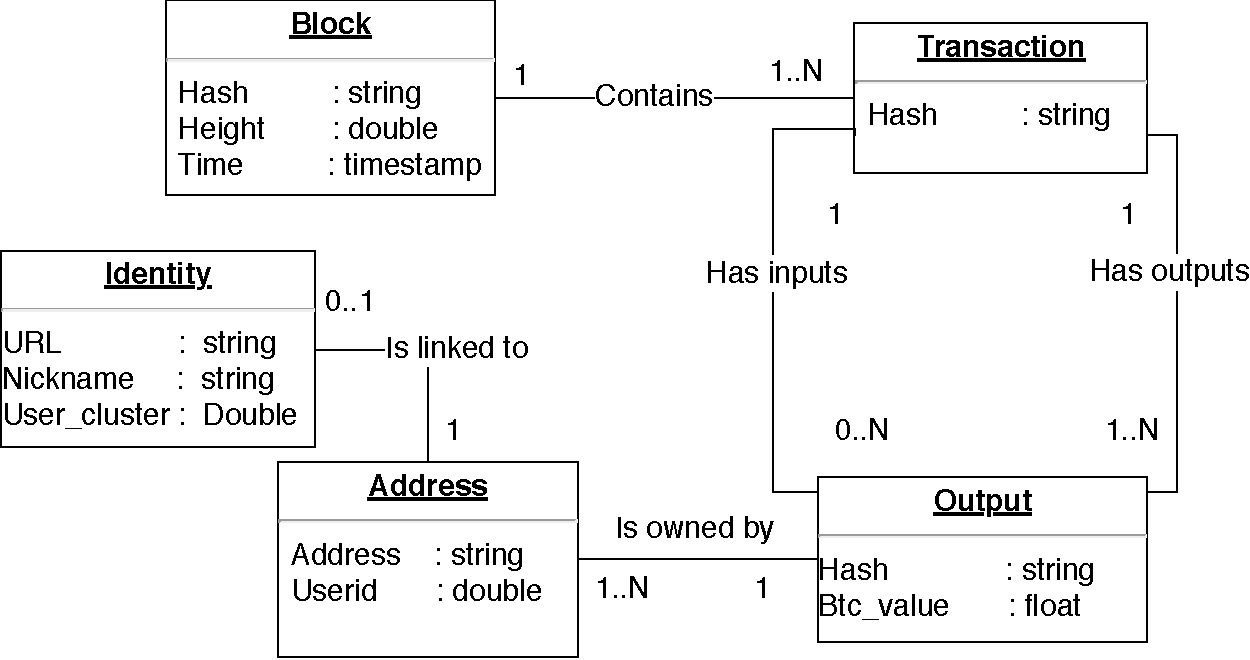
\includegraphics[width=1\textwidth]{neo4j-schema}
    \caption{Neo4j database ER diagram}
    \label{neo4jschema}
\end{figure}
XXX - dodelat

\section{Using own transactions to identify market wallets}

Valhalla cryptomarket generates uniue deposit address for each new user.
When user wants to buy something, he needs to deposit bitcoins to deposit address,
that will top up hi account balance and he used this account balance to buy stuff.
Vendor or user can request withdrawing their bitcoins from cryptomarket and so
the cryptomarket decrease their account balance and sends bitcoin to user's address.

For identifying bitcoin addresses that are owned by Valhalla cryptomarket, we 
deposited 0.05 Bitcoins to our user account on Valhalla cryptomarket and immidiatelly
performed multiple withdraws by smaller amount to recieve bitcoins back.
When we requested bitcoin withdrawals, we recieved bitcoins from different address
than the deposit one. We consider the deposit address and all addresses we recieved
bitcoins from during withdrawals owned by cryptomarket.

Detecting just these addresses would no help us detect
if someone sent or recieved bitcoins from Valhalla cryptomarket.
Cryptomarkets use thousands of bitcoin addresses and
bitcoin tumblers in order to obstruct analysis of blockchain data
that aims to identify cryptomarket's users and administrators.
In order to address this issue, we used two heuristics, that were widely used
in previous works \parencite{androulaki2013evaluating}\parencite{reid2013analysis}
for clustering bitcoin addresses belonging to same user.

The first heuristics simply states, that all inputs of one transaction belong to same user. This is logical,
since users generally don't share their private keys and collaborate on creating one transaction.
Inputs of one transaction have different bitcoin addresses, so we can check all inputs of any transaction
owned by these addresses and find new 

The second heuristics focus on detecting change address, as it was described in chapter XXX.
If transaction has two outputs with two different addresses, when one address was used and one not,
than we can safely assume, that the not used address is a change address belonging to the same user \parencite{androulaki2013evaluating}.

We labeled each address in our blockchain transaction graph with unique user number
and alternately run first and second heuristics until there were no changes in the user number property of addresses.
Both of these heuristics are pretty strict and have just a negligible chance of falsely merging
addresses not belonging to the same user.
There exist few proposals for anonymization methods that could make
these heuristics missleading( like CoinJoin and dark wallet), but
these are just concepts or in experimental alpha versions, not easily
used by even advanced users.

\chapter{Statistics of Valhalla cryptomarket}

% \section{Overall statistics of Valhalla drug market}

We managed to scrape 25309 vector listings from 981 vendors and 6381 feedbacks.
There were 17314(68\%) listings related to selling drug substances.
Vendors had from 1(90 vendors) to 1083(1 vendor)
active listings, with average of 25.69 (SD = 58.06)
and median = 11.00 listings per vendor.
The distribution can be seen in figure \ref{listingsxsellers}

\begin{figure}[!htb]
    \centering
    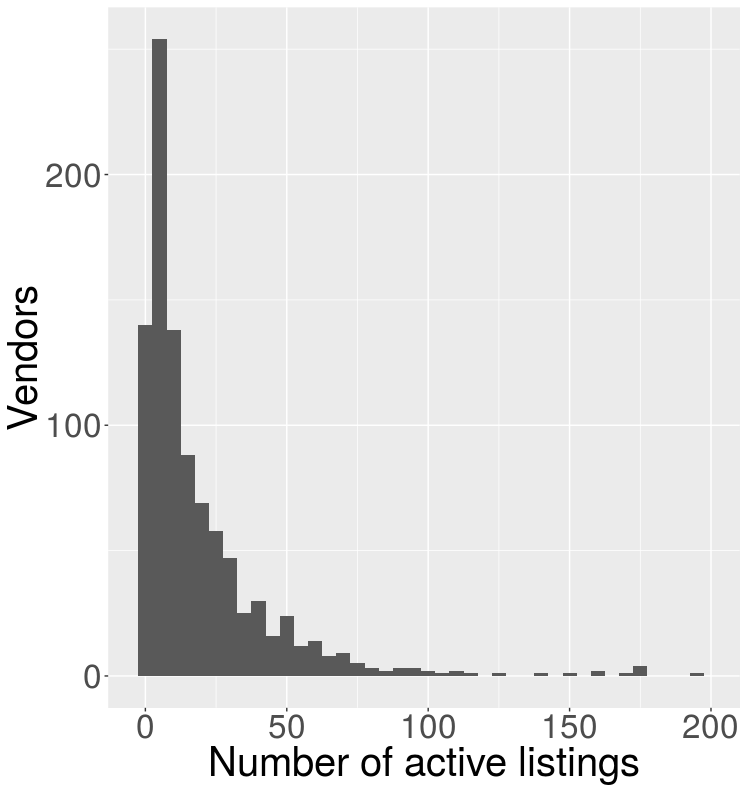
\includegraphics[scale=0.4]{listingsxsellers}
    \caption{Number of active listings for each seller}
    \label{listingsxsellers}
\end{figure}

Valhalla was originally estabilished as a local Finnish market.
That seems to be the reason for surprisingly many vendors shipping from Finland.
Vendors were shipping drugs from 39 distinct countries,
the frequency of countries the vendors were shipping from is in table \ref{shipcount}.

\begin{table}
    \caption{Countries vendors are shipping from}
    \label{shipcount}
    \begin{tabular}{|l|l|}
    Countries vendors are shipping from  & Count of vendors\\
        Australia                                    & 3   \\ 
        Poland                                       & 3   \\ 
        Spain                                        & 4   \\ 
        Canada                                       & 4   \\ 
        France                                       & 5   \\ 
        Norway                                       & 5   \\ 
        Netherlands                                  & 12  \\ 
        Germany                                      & 13  \\ 
        United States                                & 16  \\ 
        United Kingdom                               & 23  \\ 
        Finland                                      & 28  \\ 
        Others                                       & 31   \\
        Unknown                                      & 834  
    \end{tabular}
\end{table}


In the graph \ref{listingxprice} is shown distribution of prices of all listings in
 the market. 
 The graph \ref{flistingxprice} show distribution of prices gathered
 from vendor feedbacks. The \ref{flistingxprice} might count one listing
 multiple times, as one listings might be bought several times
 and therefore appear multiple times in feedback. We expect, that distribution
 of prices in these feedbacks reflects more accuratelly the prices of the goods or services
 that are actually bought at market.
 The average price of listing is 336.2 Eur(1368.2 SD!) with median of 71.Eur,
 while for feedbacks, it is 82.7Eur(150.7 SD) with median of 55 Eur.
  There were only 22(0.3\%) feedbacks with price > 1000EUR
 with only 5(0.01\%) feedbacks with price > 2000 Eur.
  For listings, there were 1533(6.05\%) active listings
 with price greater than 1000 EUR
 673(2.7\%) of them with price greater than 3550, while
 The titles of high prices listings don't indicate that 
 these listings are somehow special expect it's price.
 These findings indicate, that buyers tend to buy
 cheaper listings. The average price of the bought goods (82.7 EUR)
 is way below the emount someone who resale drugs would buy at one deal.
 There were 115 listings with zero price on the market,
 but no one of them was mantioned in feedbacks.
 The listings with 0 price had titles like "CARDING SERVICE *FREE*",
 "Custom order", "Free Carding Tutorial 2017" and "FREE SAMPLE 84\% MDMA CRYSTAL ROCKS"

\begin{figure}[!htb]
    \centering
    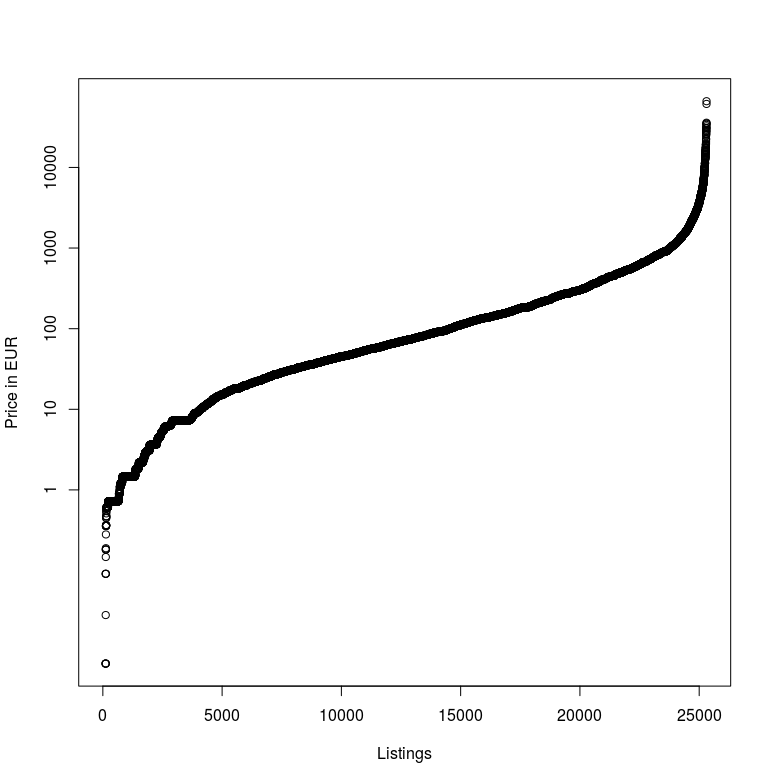
\includegraphics[scale=0.4]{listingxprice}
    \caption{Prices of listings}
    \label{listingxprice}
\end{figure}

\begin{figure}[!htb]
    \centering
    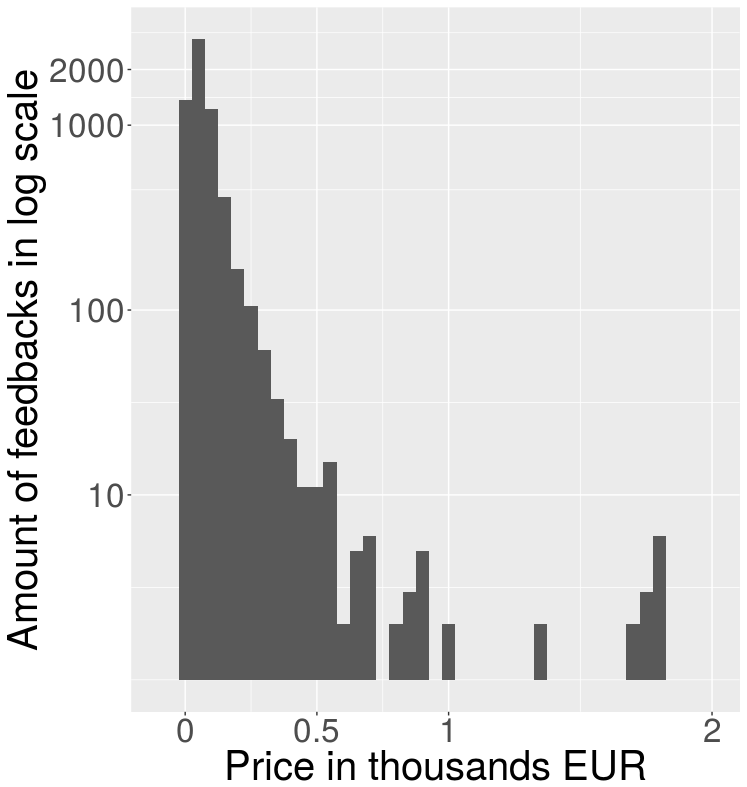
\includegraphics[scale=0.4]{flistingxprice}
    \caption{Prices of listings in feedbacks}
    \label{flistingxprice}
\end{figure}

We estimated the total revenue for each category
by summing up the prices of feedbacks.
This revenue is therefore a minimal revenue, as feedback can be given only if the
trade happened on cryptomarket.
Market share is a revenue of category divided by total revenue from all categories.

\begin{table}
    \caption{Estimated monthly revenue for selected drug categories a by listing price}
    \label{categories}
    \begin{tabular}{|l|l|l|l|l|}
Category & listings & feedbacks & revenue & market share \\
Cannabis & 5139 & 188 & 135693 & 27.6\% \\
Stimulants & 3493 & 1043 & 108157 & 22\% \\
Opiates & 1662 & 489 & 83135 & 16.9\% \\
Pharmacy & 2294 & 1104 & 62054 & 12.6\% \\
Body building & 679 & 402 & 31466 & 6.4\% \\
Empathogens & 2988 & 394 & 20344 & 4.1\% \\
Other drugs &  774 & 173 & 14350 & 2.9\% \\
Psychedelics & 1377 & 198 & 11796 & 2.4\% \\
Other products &  782 & 89 & 9106 & 1.8\% \\
Self-defence &  513 & 4 & 4635 & 0.9\% \\
Services & 1662 & 35 & 4061 & 0.8\% \\
Dissociatives &  290 & 38 & 2317 & 0.5\% \\
Classifieds &  649 & 18 & 2182 & 0.4\% \\
Cannabis growing &  56 & 2 & 44 & 0\% \\
Depressants &   71 & 2 & 59 & 0\% \\
Digital items & 2497 & 9 & 141 & 0\% \\
Mushroom growing &   26 & 2 & 178 & 0\% \\
Paraphernalia  &  36 & 0 & 0 & 0\% \\
Production / distribution &   17 & 0 & 0 & 0\% 
    \end{tabular}
\end{table}

Each circle in \ref{posneg} represents one vendor and axes represent
the number of positive and negative feedbacks that vendor recieved. 
We can see, that vast majority only 2 vendors out of 666 have recieved more negative feedback than positive.
Only 19 vendors out of 666 managed to get more than 50 negative feedbacks, while all of the these 19 vendors had more
 than 400 positive reviews.
Only 40 vendors got more negative feedbacks than positive feedbacks.
 If we look at statistics of reviews from popular e-shop amazon(http://minimaxir.com/2017/01/amazon-spark)
 and consider one and two star reviews as negative, we can see, that amazon sellers on
 average gets between 5-25\% negative reviews, depending on category of the goods.
 On the Valhalla market, vast majoririty of sellers have >95\% of positive reviews, as is shown on \ref{pospercent}.
 Also, only 40 vendors have less than 80\% positive reviews and out of that 36 have less 50 reviews in total.
 These numbers indicate, that the customers of Valhalla market
 are much more picky about the vendor they choose than regular e-shop cuystomers. If \ref{Vendors by total revenue}
  

\begin{figure}[!htb]
    \centering
    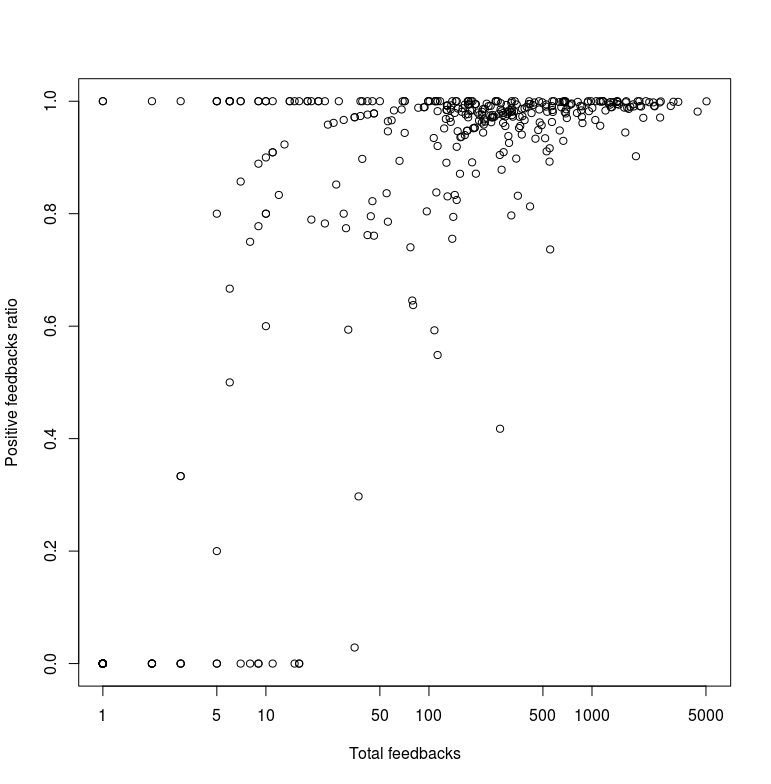
\includegraphics[scale=0.4]{posratxtotal}
    \caption{Positive reviews of vendors}
    \label{posratxtotal}
\end{figure}

\begin{figure}[!htb]
    \centering
    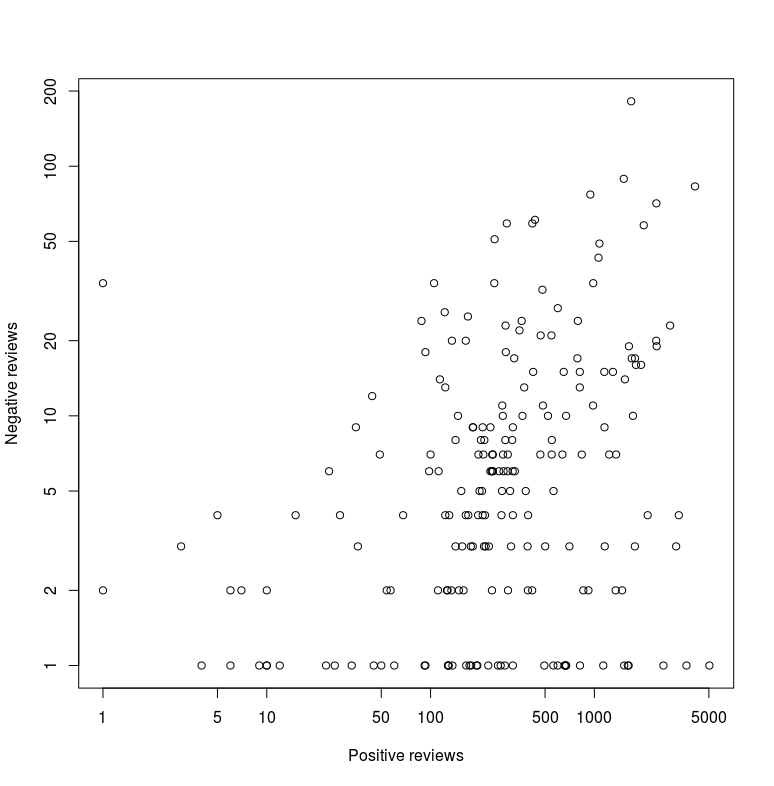
\includegraphics[scale=0.4]{posneg-log}
    \caption{Positive/negative reviews of vendors}
    \label{posneg}
\end{figure}
asfd
\begin{figure}[!htb]
    \centering
    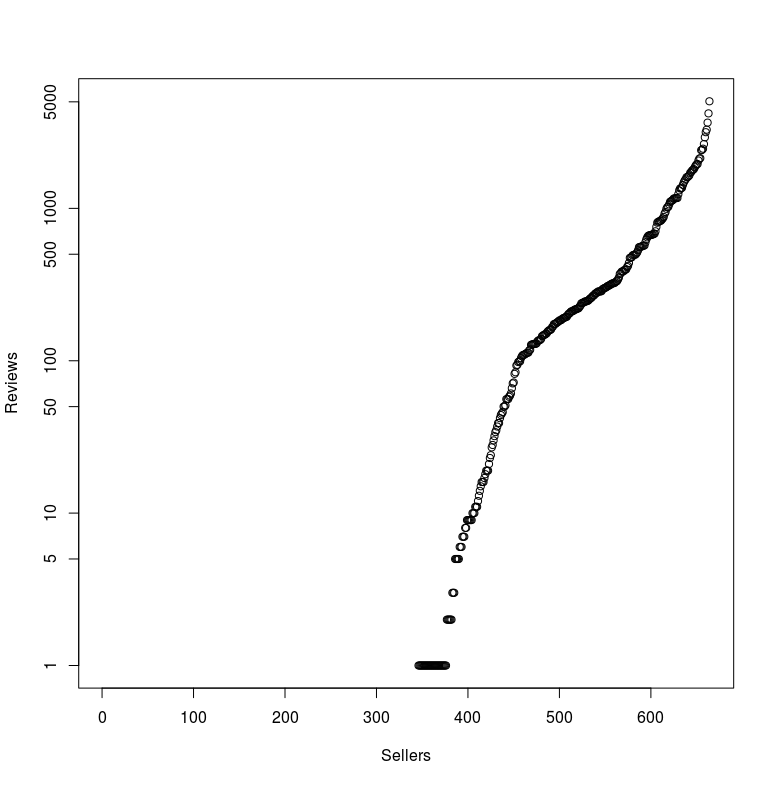
\includegraphics[scale=0.4]{reviews-count-log}
    \caption{Number of reviews for vendors}
    \label{reviews}
\end{figure}
asdf
\begin{figure}[!htb]
    \centering
    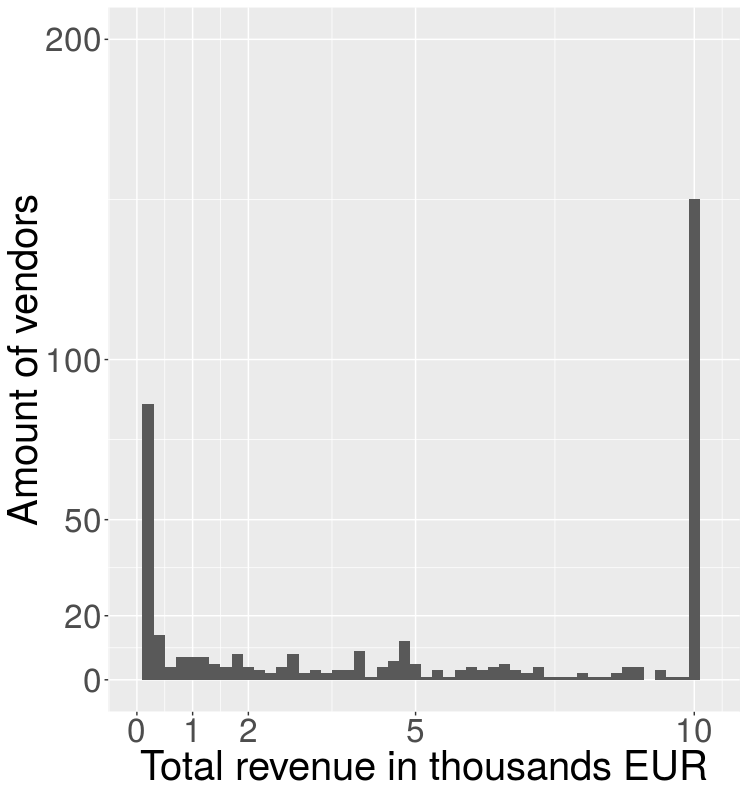
\includegraphics[scale=0.4]{total-rev}
    \caption{Total revenue of vendors}
    \label{Vendors by total revenue}
\end{figure}

% \section{Statistics about vendors, drugs availability and distribution and buyers satisfaction}


\chapter{Application}

This chapter describes the application for searching in gathered data.
The application consists of three parts.

\begin{itemize}
 \item The scraping module, that downloads bitcoin blockchain and also scrapes data from publicly available sites mentioned in section XXX.
 \item The computanional module, which imports data to the database, create indexes and compute heuristics from chapter XXX.
 \item The web GUI written in HTML/JS/CSS for sending requests to webserver and visualisation of retrieved data. 
 \item Webserver, that handles GUI requests and retrieve data from database.
\end{itemize}

\begin{figure}[!htb]
    \centering
    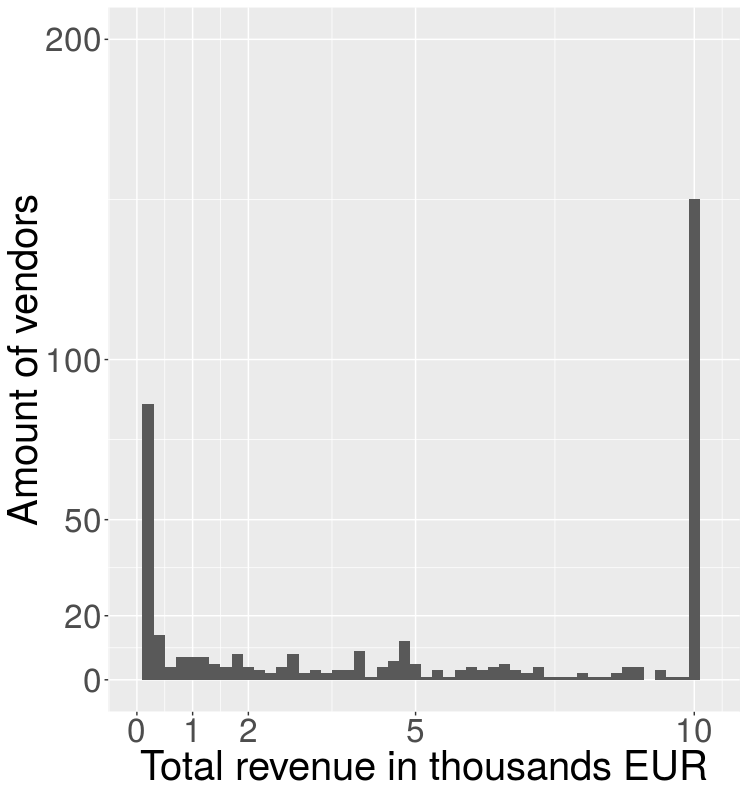
\includegraphics[scale=0.4]{total-rev}
    \caption{Application architecture}
    \label{Vendors by total revenue}
\end{figure}



\section{Implementation}

The importing module is responsible for parsing bitcoin blockchain files and importing the data into neo4j database.
The importing module take two parameters, the directory of .blk files, which store blockchain data and directory for cre
ating neo4j graph database.
The import module firstly parses the .blk files and save blockchain as multiple .csv files. This intermidiary step is us
eful for debugging and also simplifies importing to neo4j database.

\begin{figure}[!htb]
    \centering
    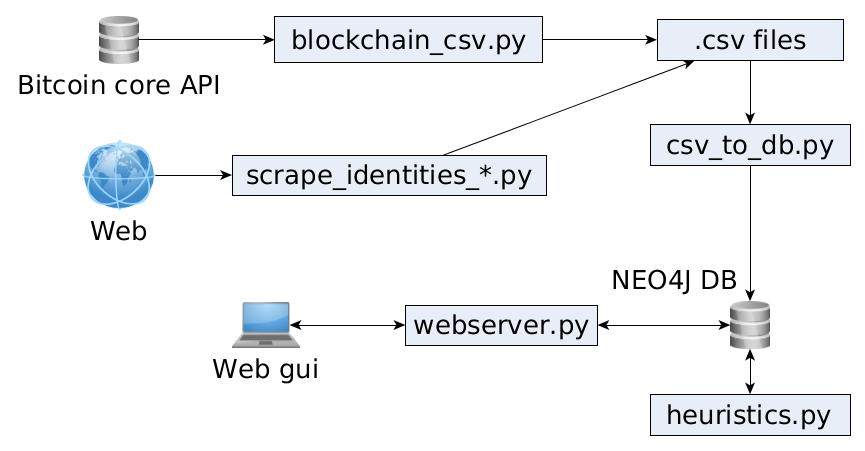
\includegraphics[width=1\textwidth]{application_architecture}
    \caption{Neo4j database ER diagram}
    \label{application_architecture}
\end{figure}

The next importing script is scrape\_identities.py script, which crawl popular forums and multiple websites and creates 
identities.csv.
File identities.csv contains 3 collumns.
\begin{itemize}
  \item Address - bitcoin address the identity is associated with
  \item Identity - String representing identity, usually username
  \item URL - Url where the Identity and Address were scraped
\end{itemize}

If the user has his own data about the owners of different bitcoin addresses, he can import it through the web GUI later
.


\section{Usage}

\noindent See the following command :
\begin{lstlisting}[language=bash]
  $ ./import_module ~/.blockchain/ ~/neo4j/graph.db
\end{lstlisting}

\section{Future development possibilities}


\chapter{Testing and verification of the created tool}
This chapter describes the way, the POC application was tested.

The testing were performed by sending bitcoins to drug markets and withdrawing them.
Than marking the addresses from where the bitcoins were received as 'a
\section{Method of testing}
\section{results}



\chapter{Conclusion}

Here you can insert the appendices of your thesis.gg

\printbibliography
\end{document}
